\section{Домашнее задание}
\addcontentsline{toc}{section}{Домашнее задание}	% Добавляем его в оглавление

\begin{figure}[h]
\begin{center}
  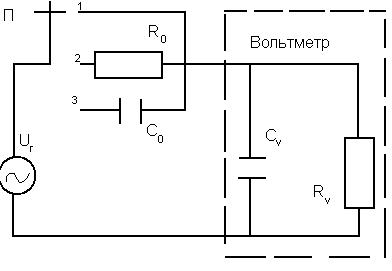
\includegraphics[width=0.3\linewidth]{scheme1}
  \caption{Исходная схема\label{sch1}}
\end{center}
\end{figure}

\begin{table} [htbp]
  \centering
  \begin{tabular}{| p{3cm} | p{3cm} | p{1.5cm} | p{1.5cm} | p{1.5cm} | p{3cm}l |}
  \hline
  \centering № варианта &\centering Линейное напряжение, В &\multicolumn{3}{c|}{Количество элементов в фазе} &\centering Регулируемая фаза & \\ \cline{3-5}

  & &\centering Фаза А &\centering Фаза Б &\centering Фаза С & & \\ 
  \hline

  \centering 4 &\centering 33 &\centering 7 &\centering 5 &\centering 3 &\centering A & \\
  \hline

  \end{tabular}
  \caption{Данные для расчета}
\end{table}

\begin{enumerate}
\item Для трёхфазной трёхпроводной цепи (рис. ~\ref{sch1}) по данным из таблицы:

\begin{itemize}
\item Определим напряжение между нулевыми узлами:\par

\begin{minipage}[h]{0.65\linewidth}

$ \dot{U}_{AB} = 33*e^{j30^{\circ}} = 28.759 + 16,500j $ (В)

\vspace{2mm}

$ \dot{U}_{BC} = 33*e^{-j90^{\circ}} = -33j $ (В)

\vspace{2mm}

$ \dot{U}_{CA} = 33*e^{j150^{\circ}} = -28.579 + 16,500j $ (В)

\vspace{2mm}

$ \dot{U}_{A} = U_{f} = 19,053 $ (В) 

\vspace{2mm}

$ \dot{U}_{B} = U_{f}*e^{-j120^{\circ}}  = -9,526 - 16,5j $ (В)

\vspace{2mm}

$ \dot{U}_{C} = U_{f}*e^{j120^{\circ}}  = -9,526 + 16,5j $ (В)

\vspace{2mm}



\end{minipage}    
\hfill
\begin{minipage}[h]{0.35\linewidth}

$ U_{l} = 33 $ (В); \hspace{4mm} $ Z = 280 $ (Ом)

\vspace{2mm}

$ U_{f} = \dfrac{U_{l}}{\sqrt{3}} = 19,053 $ (В)

\vspace{2mm}

$ Y_{A} = \dfrac{7}{Z} = 25*10^{-3} $ (См) 

\vspace{2mm}

$ Y_{B} = \dfrac{5}{Z} = 17,86*10^{-3} $ (См) 

\vspace{2mm}

$ Y_{C} = \dfrac{3}{Z} = 10,7*10^{-3} $ (См) 

\end{minipage}

\begin{center}
$ \dot{U}_{Nn} = \dfrac{\dot{U_{A}}Y_{A} + \dot{U_{B}}Y_{B} + \dot{U_{C}}Y_{C}}{Y_{A} + Y_{B} + Y_{C} } = 3,814 - 2,206j $ (В)
\end{center}

\vspace{2mm}

\item Определим напряжение каждой фазы нагрузки:
\begin{center}

$ \dot{U}_{a} = \dot{U}_{A} - \dot{U}_{Nn} = 19,053 - 3,814 + 3,206j = 15,239 + 3,206j $

\vspace{2mm}

$ \dot{U}_{b} = \dot{U}_{B} - \dot{U}_{Nn} = 9,526 - 16,5j - 3,814 + 3,206j = -13,340 - 13,294j $

\vspace{2mm}

$ \dot{U}_{c} = \dot{U}_{C} - \dot{U}_{Nn} = 9,526 + 16,5j - 3,814 + 3,206j = -13,340 + 19,706j $

\end{center}

\item Определим ток в каждой фазе:
\begin{center}
$ \dot{I}_{a} = \dot{U}_{a}Y_{a} = (15,239 + 3,206j) * 25 \cdot 10^{-3} = 0,381 + 0,080j = 0,389 * e^{j11,858^{\circ}} $ (A) 

\vspace{2mm}

$ \dot{I}_{b} = \dot{U}_{b}Y_{b} = (-13,340 - 13,294j) * 17,86 \cdot 10^{-3} = -0,238 - 0,237j = 0,336 * e^{j135,12^{\circ}} $ (A) 

\vspace{2mm}

$ \dot{I}_{c} = \dot{U}_{c}Y_{c} = (-13,340 + 19,706j) * 10,7 \cdot 10^{-3} = -0,143 + 0,211j = 0,255 * e^{j124,13^{\circ}} $ (A) 
\end{center}

\vspace{2mm}

\item Определим активную мощность, потребляемую цепью:
\begin{center}

$ P_{1} = \vert \dot{U}_{AB} \vert \vert \dot{I}_{a} \vert \cos{(\varphi_{U_{AB}} - \varphi_{I_{A}})} = 12,199 $ (Вт)

\vspace{2mm}

$ P_{2} = \vert \dot{U}_{CB} \vert \vert \dot{I}_{c} \vert \cos{(\varphi_{U_{CB}} - \varphi_{I_{C}})} = 6,966 $ (Вт)

\vspace{2mm}

$ P = P_{1} + P_{2} = 19,165 $ (Вт)

\end{center}
\item По данным расчёта построим векторную диаграмму:

\vspace{70mm}

\end {itemize}


\item Для трёхфазной четырехпроводной цепи:

\begin{itemize}
\item Выполним расчет токов и напряжений:\par
\begin{minipage}[h]{0.45\linewidth}

$ U_{Nn} = 0 $

\vspace{2mm}

$ \dot{U}_{a} = \dot{U}_{A} = 19,053 $ (В)

\vspace{2mm}

$ \dot{U}_{b} = \dot{U}_{B} = -9,526 - 16,5j $ (В)

\vspace{2mm}

$ \dot{U}_{c} = \dot{U}_{C} = -9,526 + 16,5j $ (В)


\end{minipage}
\hfill
\begin{minipage}[h]{0.45\linewidth}

$ \dot{I}_{A} = \dot{U}_{a} Y_{a} = 0,476*e^{j0^{\circ}} $

\vspace{2mm}

$ \dot{I}_{B} = \dot{U}_{b} Y_{b} = 0,34*e^{-j120^{\circ}} $

\vspace{2mm}

$ \dot{I}_{C} = \dot{U}_{c} Y_{c} = 0,204*e^{j120^{\circ}} $

\vspace{2mm}

$ \dot{I}_{N} = \dot{I}_{A} + \dot{I}_{B} + \dot{I}_{C} = 0,118*e^{-j90^{\circ}}$

\end{minipage}
\vspace{2mm}

\begin{center}

$ P_{1} = \vert \dot{U}_{AB} \vert \vert \dot{I}_{a} \vert \cos{(\varphi_{U_{AB}} - \varphi_{I_{A}})} = 13,6 $ (Вт)

\vspace{2mm}

$ P_{2} = \vert \dot{U}_{CB} \vert \vert \dot{I}_{c} \vert \cos{(\varphi_{U_{CB}} - \varphi_{I_{C}})} = 5,83 $ (Вт)

\vspace{2mm}

$ P = P_{1} + P_{2} = 19,43 $ (Вт)

\end{center}

\item По данным расчёта построим векторную диаграмму:

\vspace{70mm}

\end {itemize}

\end{enumerate}
